\chapter{結果と考察}

\section{実験結果と考察}
\ref{plan}節で示した実験計画に従って評価実験を行った.
以下では,実験協力者2名について,それぞれのタスクの取り組みや,ドキュメントとソースコードの乖離検知をしたときの行動を詳細にまとめる.

\subsection{前半に提案ツールを使用した実験協力者}
前半に提案ツールを使用した実験協力者(以下,実験協力者Aと呼ぶ)の行動と乖離検知の流れを図\ref{usera}に示す.
実験協力者Aは,タスク1ではドキュメントを更新せずにソースコードの追加のみを行っていた.
このとき,


その後の後半タスクでは,前半に乖離検知の通知を受け取ったことを受けて,タスクに取り組むときは,ドキュメントとソースコードの両方を追加・修正しており,
ドキュメントとソースコードが乖離することはなかった.

\begin{figure}[H]
    \centering
    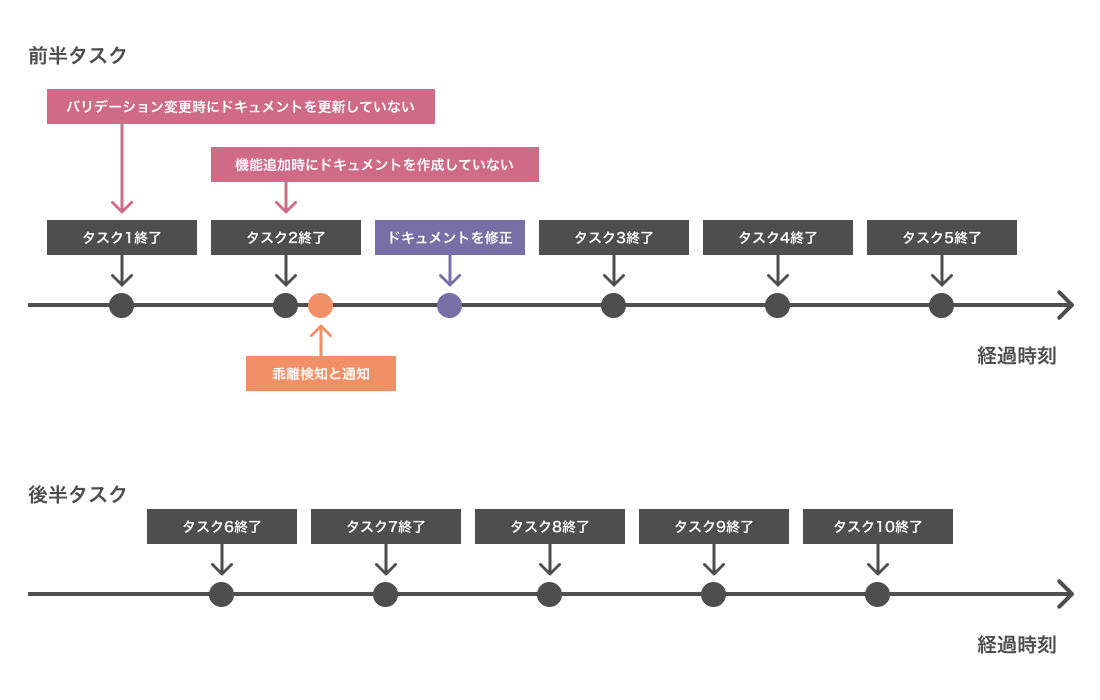
\includegraphics[width=8cm]{images/UserA.png}
    \caption{前半に提案ツールを使用した実験協力者の行動と乖離検知の流れ}
    \label{usera}
\end{figure}

\subsection{後半に提案ツールを使用した実験協力者}

\begin{figure}[H]
    \centering
    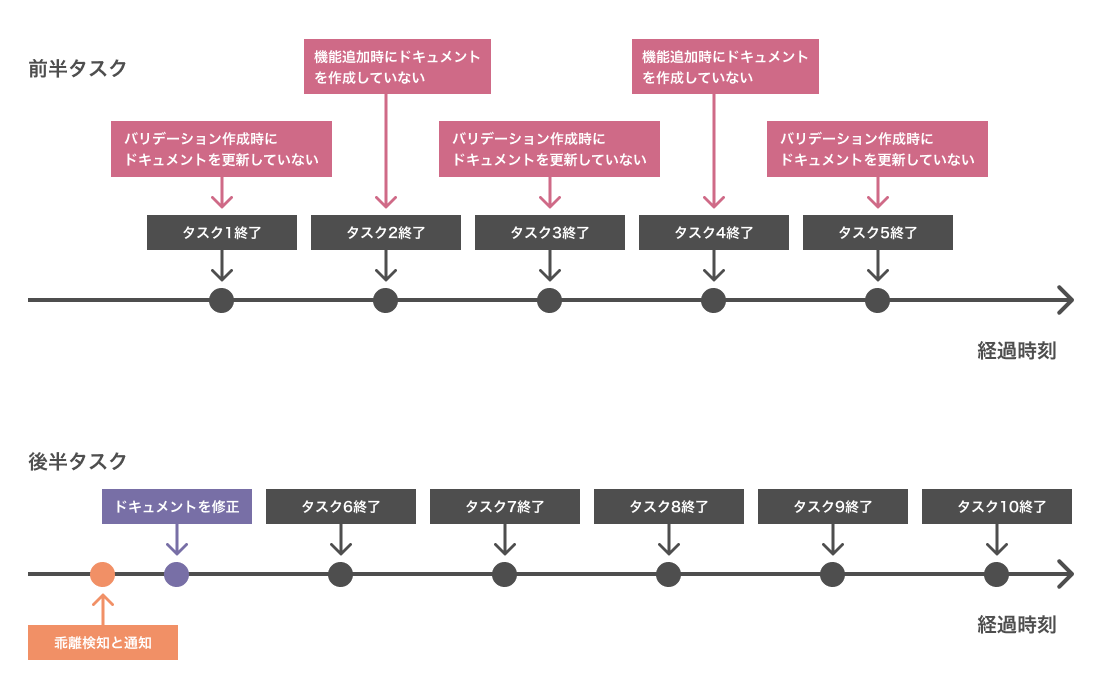
\includegraphics[width=8cm]{images/UserB.png}
    \caption{後半に提案ツールを使用した実験協力者の行動と乖離検知の流れ}
    \label{userb}
\end{figure}

\section{アンケート結果と考察}